\chapter{Exploring $N = 2$ with a Forward-Euler Algorithm}

\section{Choosing an Algorithm}

\abc

\carol
Now that we have the equations of motion for the relative position of
one particle with respect to the other, I guess we need an algorithm
to integrate these equations.

\alice
Indeed, and there is a large choice!  If you pick up any book on
numerical methods, you will see that you can select from a variety of
lower-order and higher-order integrators, and for each one there are
additional choices as to the precise structure of the algorithm.

\bob
What is the order of an algorithm?

\alice
It signifies the rate of convergence.  Since no algorithm with a
finite time step size is perfect, they all make numerical errors.
In a fourth-order algorithm, for example, this error scales as the
fourth power of the time step -- hence the name fourth order.

\carol
If that is the case, why not take a tenth order or even a twentieth
order algorithm.  By only slightly reducing the time step, we would
read machine accuracy, of order $10^{-15}$ for the usual double
precision (8 byte, i.e. 64 bit) representation of floating point numbers.

\alice
The drawback of using high-order integrators is two-fold: first, they
are far more complex to code; and secondly, they do not allow arbitrarily
large time steps, since their region of convergence is limited.  As a
consequence, there is an optimal order for each type of problem.  When
you want to integrate a relatively well-behaved system, such as the
motion of the planets in the solar system, a twelfth-order integrator
may well be optimal.  Since all planets follow well-separated orbits,
there will be no sudden surprises there.  But when you integrate a
star cluster, where some of the stars can come arbitrarily close to each
other, experience shows that very high order integrators lose their edge.
In practice, fourth-order integrators turn out to be optimal for the job.

\bob
How about starting with the lowest-order integrator we can think off?
A zeroth-order integrator would make no sense, since the error would
remain constant, independent of the time step size.  So the simplest
one must be a first-order integrator.

\alice
Indeed.  And the simplest version of a first-order integrator is
called the {\it forward Euler\ } integrator.

\bob
Was Euler so forward-looking, or is there also a {\it backward Euler\ }
algorithm?

\alice
There is indeed.  In the forward version, at each time step you simply
take a step tangential to the orbit you are on.  After that, at the
next step, the new value of the acceleration forces you to slightly
change direction, and again you move for a time step $dt$ in a straight
line in that direction.  Your approximate orbit is thus constructed
out of a number of straight line segments, where each one has the
proper direction at the beginning of the segment, but the wrong one at
the end.

\bob
And the {\it backward Euler} algorithm must have the right direction
at the end of a time step, and the wrong one at the beginning.  Let's
see.  That seems much harder to construct.  How do you know at the
beginning of a time step in what direction to move so that you come
out with the right direction tangential to a correct orbit at that
point?

\alice
You can only do that through iteration.  You guess a direction, and
then you correct for the mistake you find yourself making, so that
your second iteration is much more accurate, in fact first-order
accurate.  Given this extra complexity, I suggest that we start with
the forward Euler algorithm.

\carol
Can't we do both, \ie make half the mistakes of each of the two, while
trying to strike the right balance between forward and backward Euler?

\alice
Aha!  That is a good way to construct better algorithms, which then
become second-order accurate, because you have canceled the first-order
errors.  Examples are second-order Runge Kutta, and leapfrog.  We'll
soon come to that, but for now let's keep it simple, and stay with
first order.  Here is the mathematical notation:

\begin{eqnarray}
\br_{i+1} & = & \br_i + \bv_i dt \label{forward-euler-step1} \\
\bv_{i+1} & = & \bv_i + \ba_i dt \label{forward-euler-step2}
\end{eqnarray}

for the position $\br$ and velocity $\bv$ of an individual particle,
where the index $i$ indicates the values for time $t_i$ and $i+1$ for
the time $t_{i+1}$ after one more time step has been taken:
$dt = t_{i+1} - t_i$.  The acceleration induced on a particle by the
gravitational forces of all other particles is indicated by $\ba$.
So, all we have to do now is to code it up.  By the way, let's rename
the file.  Rather than a generic name {\st nbody.C}, let's call it
{\st forward\_euler1.C}.

\bob
Alice, go for it!

\cba

\section{Writing a Code}

After some further discussion among the three, here is the code that
Alice typed in.  Actually, the first version contained a few errors,
not surprisingly, but to speed up a bit, we will just show here the
final product, by printing the file {\st forward\_euler1.C}:

\code{forward\_euler1.C}{chap3/forward_euler1.C}

Let us look at each line in turn.  The first {\st \#include} statement
is needed in C++ in order to gain access to the I/O library, to make
sense of output statements like {\st ``cout <<''} at the end of the
code.  The second {\st \#include} statement gives access to the math
library that contains functions such as the square root {\st sqrt()}.
The third line is a default C++ way of indicating that we use the
standard name space.  Later, when our software environment will have
grown significantly, it will make sense to introduce our own name
spaces, but for now the default choice suffices.

There is only one function in this file, the {\st main()} function
which has to be present in every C++ program.  It is defined as type
{\st int}, which means that it returns an integer value (by default
defined to be 0 upon successful completion, and nonzero otherwise).
The three arrays {\st r[3], v[3], a[3]} store the values for the
three Cartesian components of the relative position, velocity and
acceleration of one particle with respect to the other.  These are
declared as {\st double}, the C++ way to indicate 8-byte floating
point variables.

In this simple program there is no need for any input: all initial
values are chosen already in the program.  The time step {\st dt} is
fixed to be $0.01$.  The relative position is chosen along the $x$
axis at a distance of unity from the origin where the other particle
resides in the relative coordinate system that we use.  The velocity
is chosen to be $0.5$ in the direction of the positive $y$ axis.  This
is less than the value $v_y = 1$ needed to sustain a circular orbit,
as you can check in any book on celestial mechanics or stellar
dynamics.  The choice of a velocity less than the circular velocity
means that we have captured the relative motion at apocenter, which is
the point in the orbit at which the two particles are furthest away
from each other.  The word is derived from the Greek $\alpha \pi o$
{\it (apo)} meaning `far (away) from'.  The subsequent motion will
bring the two particles closer together, until the pericenter is
reached on the negative $x$ axis, which is the point in the orbit at
which the two particles are closest.  This word is derived from the
Greek $\pi \epsilon \rho \iota$ {\it (peri)} meaning `around' or
`near'.  After passing through pericenter the particles will move away
from each other again.

The {\st for} loop takes 1000 time steps that are counted by the
variable {\st ns}, covering a time interval of 10 units.  The body of
the loop shows how we first compute the square of the scalar distance
between the two particles by summing the squares of the Cartesian
components.  We then take the square root, and multiply that with the
square of the distance to get the third power of the distance, which
we have seen in the denominator of Eq. \ref{newton-2-bodies} on
p.~\pageref{newton-2-bodies}, which we repeat here for convenience:

\begin{equation}
\frac{d^2}{dt^2}\br = - \frac{\br}{r^3}
\end{equation}

\noindent
In our code we find this equation back in component form as:

\begin{small}
\begin{verbatim}
        a[k] = - r[k] / (r2 * sqrt(r2))
\end{verbatim}
\end{small}

Finally, the integration step is completed by executing
Eqs. \ref{forward-euler-step1}, \ref{forward-euler-step2} on
p.~\pageref{forward-euler-step1} above, to update the relative
position and velocity.  At the end of each time step, we print the
three position and three velocity components, all on a single line.

To compile the code, we must invoke a C++ compiler.  In a Linux
environment, the natural compiler is the GNU C++ compiler that is
called by the {\st g++} command:

\begin{small}
\begin{verbatim}
g++ -o forward_euler1 forward_euler1.C
\end{verbatim}
\end{small}

which will produce an executable file {\st forward\_euler1}, if no
errors are detected during compilation.  Let us follow the discussion
of our three friends, from the moment that their code first compiled.

\section{Running a Code}

\abc

\carol
That's it, the last bug caught, our {\st forward\_euler1} compiled at
last!  Let's see what it produces.  Since we asked for the output of
positions and velocities for 10 time units at intervals {\st dt = 0.01},
our screen will be flooded by 1000 lines of output; better to redirect
the output to a file.  Let's call it {\st forward.out}, and let's have
a look at the beginning and the end of the file, say five lines each:

\cba

% \begin{Output}
% \begin{small}
% \begin{verbatim}
% |gravity> forward_euler1 > forward.out
% |gravity> head -5 forward.out
% 1 0.005 0 -0.01 0.5 0
% 0.9999 0.01 0 -0.0199996 0.49995 0
% 0.9997 0.0149995 0 -0.0300001 0.49985 0
% 0.9994 0.019998 0 -0.0400027 0.4997 0
% 0.999 0.024995 0 -0.0500088 0.4995 0
% |gravity> tail -5 forward.out
% 7.66125 -6.25475 0 0.812523 -0.574458 0
% 7.66937 -6.26049 0 0.812443 -0.574393 0
% 7.6775 -6.26623 0 0.812364 -0.574329 0
% 7.68562 -6.27198 0 0.812286 -0.574264 0
% 7.69375 -6.27772 0 0.812207 -0.5742 0
% |gravity>
% \end{verbatim}
% \end{small}
% \end{Output}
\output{chap3/forward.output}
\abc

\bob
Hey, Alice told us that our two particles were at apocenter initially,
at distance 1, which meant that they could come closer but that they
would never get further away from each other than unity in our length
units.  And here we have distance vectors larger than 7, actually
close to 10 if I remember my Pythagoras formula well enough, in the
last line.

\carol
You are right, slightly more than 9.9:

\cba

\begin{small}
\begin{verbatim}
|gravity> bc
7.69375*7.69375 + 6.27772*6.27772
98.6035574609
sqrt(98.6035574609)
9.92993239961380603154
|gravity>
\end{verbatim}
\end{small}

\abc

\bob
Unix takes a while to get used to!  What does the two-letter `word'
{\st bc} mean?

\carol
Oh, {\st bc} is a more powerful version of {\st dc}, which stands for
`desk calculator' and is a simple utility to quickly find arithmetic
answers without writing a program.  Here is what the manual page for
{\st dc} tells us:

\cba

\begin{small}
\begin{verbatim}
|gravity> man dc
NAME
     dc - desk calculator

SYNOPSIS
     dc  [ filename ]

DESCRIPTION
     dc  is an arbitrary  precision  arithmetic  package.   Ordi-
     narily  it operates on decimal integers, but one may specify
     an input base, output  base,  and  a  number  of  fractional
     digits  to  be maintained. The overall structure of dc  is a
     stacking (reverse Polish) calculator.   If  an  argument  is
     given,  input  is  taken  from that file until its end, then
     from the standard input.

     bc  is a preprocessor for dc  that provides  infix  notation
     and  a  C-like  syntax  that implements functions.  bc  also
     provides reasonable control  structures  for  programs.  See
     bc(1).
|gravity>
\end{verbatim}
\end{small}

\abc

\carol
With {\st dc} we could not have used the {\st sqrt()} function, so we
used {\st bc}; perhaps it stands for a `better calculator', who knows.

\bob
Well, our program compiles and our program runs, so we have passed two
barriers, but now it gives answers that are not sensible.  The third
step that could have gone wrong is that we have somehow made a mistake
in our algorithm, mistyping it, or even being misguided as to its
structure.  But with the simplicity of Eqs. \ref{forward-euler-step1},
\ref{forward-euler-step2} it seems clear that neither is the case here.
The equations tell the particle to `follow its nose' in a straight
line during each time step.  What could be simpler!

\alice
You are right.  After syntactic compile time errors, dynamic run time
errors, and semantic errors in coding up the algorithm correctly, the
fourth potential source of errors lies in using the algorithm.  While
it seems that we took an almost ridiculously small time step, the
choice {\st dt = 0.01} may still be too large.  After all, {\st dt} is
the only free parameter in our program.  The code is like a laboratory
instrument, a black box with only one dial, so we may as well play
with different settings of the dial.

\bob
Indeed, we had no particular reason to choose the value we did, rather
than any other.  But before we start playing, can we plot a picture of
the orbit we just computed?  I'd rather have a real sense of what is
going on, beyond staring at a few output numbers.

\carol
Will do, but may I add another option to Alice's detective analysis?
Apart from the four types of error that she mentioned, there is another
possibility.  We are not really sure that the program we ran was the
one we wrote.  The default search path on this computer may be set such
that we wind up invoking another program with the same name.

\bob
Also called {\st forward\_euler1}?  That seems extremely unlikely!

\carol
But as they say in the Hitchhiker's guide to the galaxy, not impossible.
Let me try, and force execution from the current directory ``.'' by
adding it to the name of our executable:

\cba

\output{chap3/forward2.output}

\abc

\carol
Okay, no problem here.  I just thought I'd bring up something I
happened to learn in class today.  Now let's look at a picture of the
orbit.  I suggest using {\st gnuplot}, present on any Linux running
system, and something that can be easily installed on many other Unix
systems as well.  To use it is quite simple, with only one command
needed to plot a graph.  In our case, however, I'll start with the
command {\st set size ratio -1}.  A positive value for the size ratio
scales the aspect ratio of the vertical and horizontal edge of the box
in which a figure appears.  However, in our case we want to set the
scales so that the unit has the same length on both the x and y axes.
Gnuplot can be instructed to do so by specifying the ratio to be {\st -1}.
In fact, let me write the line {\st set size ratio -1} in a file called
{\st .gnuplot} in my home directory.  That way we don't have to type it
each time we use gnuplot.  Okay, done.  Now let's have our picture:

\cba

\begin{small}
\begin{verbatim}
|gravity> gnuplot
gnuplot> set size ratio -1
gnuplot> plot "forward.out"
gnuplot> quit
|gravity> 
\end{verbatim}
\end{small}

\begin{figure}[ht]
\centering
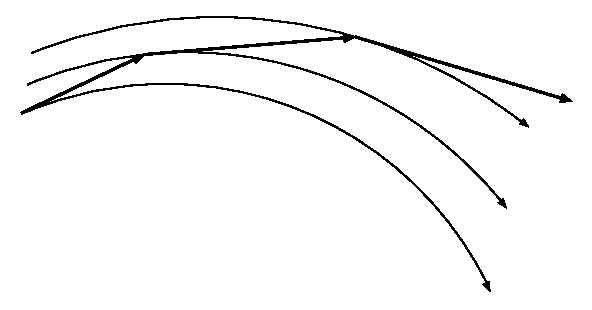
\includegraphics[width=4.5in]{chap3/forward1.ps}
\caption[Two-body orbit with a forward-Euler integrator, time step $dt = 0.01$]
{Relative orbit for the first attempt to integrate a two-body system with a
forward-Euler integrator, with time step $dt = 0.01$}
\label{fig:forward1}
\end{figure}

\abc

\bob
Wow, the two stars were flung away as by a slingshot, after only
slightly more than half an orbit.  I guess that indeed the time step
was too large.

\alice
I think you are right.  Notice that the artificial slingshot, caused
by numerical errors, occurred just after pericenter, where the
curvature of the orbit is highest.  Stepping along tangentially to the
orbit tends to let you spiral out from the original orbit, and this
effect is higher when the orbital curvature is higher.

\carol
Okay, I'll change the time step size.

\cba

\section{Extending a Code}

\abc

\carol
In addition, rather than changing the program each time we change step
size, I'll make it an option to be provided by the user.  How about
this version:

\cba

\code{forward\_euler2a.C}{chap3/forward_euler2a.C}

\abc

\bob
And even with a polite request to remind the user what is needed.
Very nice.  Let's compile, run, and plot!

\carol
Okay.  Let's direct to output to a file {\st forward2a.out}, and let's
rename the old output file {\st forward1.out}, to get a consistent
numbering system, where the number in the source file corresponds to
the same number in the output file; the `a' after `2' is added here
since different input options will produce different output files.

\bob
How about making it even clearer and add the value of the time step
that we input to the name?

\carol
Yes, even better.  Let's start with $dt = 0.01$, the same value we
used by default in {\st forward\_euler1.C}.  It never hurts to check
whether we indeed get the same result.  Here goes:

\begin{small}
\begin{verbatim}
|gravity> g++ -o forward_euler2 forward_euler2.C
|gravity> mv forward.out forward1.out
|gravity> forward_euler2 > forward2_0.01.out
\end{verbatim}
\end{small}

\bob
So much for the polite reminder.  What is happening, is the computer
so slow?  Or is it just hanging?

\alice
Ah, I see.  By redirecting the output to {\st forward2\_0.01.out}, we are
also redirecting our reminder to that file, spoiling the format of our
nbody snapshot output, and losing our reminder.

\carol
Yes, of course, you are right.  Well, how about putting the reminder
on the error stream {\st cerr}, rather than the output stream {\st
cout}?  While reminding you of something is not an error, it does
provide a handy way to disentangle the snapshot output, meant to be
read further by a computer, and the reminder output, aimed at human
consumption.

\bob
Good idea.  But while we do that, let's make another modification as
well.  I just realized that our halting criterion is completely wrong.
If we specify {\st dt = 0.0001}, the system would bail out after only
1000 steps, as before, thus advancing the time from zero to 0.1, barely
enough to see the particles move, and far too little to complete even
one orbit.

\alice
Right you are.  Let's put in a time counter, so that we can keep
integrating till time 10, for good measure.

\carol
Fine!  And I'll rename the previous version {\st forward\_euler2a.C},
while keeping the name {\st forward\_euler2.C} for the corrected version.
When you are developing code, it is always a good idea to keep older
versions lying around, even if they are wrong.  After all, subsequent
versions may turn out to be even more wrong, in which case you might
well want to go back to the less wrong one!  Here we are:

\cba

\code{forward\_euler2.C}{chap3/forward_euler2.C}

\abc

\carol
And now let's try again:

\cba

\output{chap3/forward2a.output}

% \begin{small}
% \begin{verbatim}
% |gravity> g++ -o forward_euler2 forward_euler2.C
% |gravity> forward_euler2 > forward2_0.01.out
% forward2_0.01.out: File exists.
% |gravity> rm forward2_0.01.out
% rm: remove `forward2_0.01.out'? y
% |gravity> forward_euler2 > forward2_0.01.out
% Please provide a value for the time step
% 0.01
% |gravity> tail -2 !$
% tail -2 forward2_0.01.out
% 7.69375 -6.27772 0 0.812207 -0.5742 0
% 7.70187 -6.28346 0 0.812128 -0.574136 0
% \end{verbatim}
% \end{small}

\abc

\bob
That's curious.  Almost the same results as before, but not quite.
Remember, earlier we got:

\cba

% \begin{small}
% \begin{verbatim}
% 7.68562 -6.27198 0 0.812286 -0.574264 0
% 7.69375 -6.27772 0 0.812207 -0.5742 0
% \end{verbatim}
% \end{small}

\output{chap3/forward2b.output}

\abc

\bob
Ah, I see: same results, after all, but one more time step.
Our next to last line is identical to our previous last line.

\carol
That would imply that the new file should be one line longer.  Let's
check by doing a word count (actually a line-word-character count):

\cba

% \begin{small}
% \begin{verbatim}
% |gravity> wc *.out
%    1000    6000   39633 forward1.out
%    1001    6006   39673 forward2_0.01.out
%    2001   12006   79306 total
% |gravity> 
% \end{verbatim}
% \end{small}
\output{chap3/wc.output}

\abc

\alice
Indeed: one line more and six words more, for the extra position and
velocity components.  I guess our switch from integer book keeping
with the number of time steps, to floating-point book keeping by using
the time introduced some slight round-off which caused the program to
do one more step.

\bob
Sounds plausible, but let's check it out.  Seeing is believing!
Shall we put in an extra output statement on {\st cerr}?  This time
we're after errors after all, namely round-off errors.  Let's add
the following line at the end, after the two lines starting with {\st
cout}:

\cba

\begin{small}
\begin{verbatim}
	cerr << t << endl;
\end{verbatim}
\end{small}

\abc

\carol
Done.  I'll call the resulting code {\st forward\_euler2b.C}, following
our tradition to keep all version around for a while.  Let's run the
code again, but I won't bother about the snapshot output, since we
already know what that is.  Redirecting the {\st cout} output to {\st
/dev/null} is a time-honored Unix way to get rid of it.  The `null'
device acts like a black hole, getting rid of whatever falls into it,
without a trace.  We are then left only with the {\st cerr} output on
the screen.

\cba

% \begin{small}
% \begin{verbatim}
% |gravity> g++ -o forward_euler2b forward_euler2b.C
% |gravity> forward_euler2b > /dev/null
% Please provide a value for the time step
% 0.01
% 0
% 0.01
% 0.02
% 0.03
%  . . . . . .
% 9.97
% 9.98
% 9.99
% 10
% |gravity> 
% \end{verbatim}
% \end{small}
\output{chap3/forward2b_cerr.output}
\abc

\bob
Hah!  So much for your clever theory, Alice.  It stopped at {\st t = 10},
right on the mark.  So round-off cannot have been the reason.

\alice
Not so quick in claiming victory, Bob.  Look at the code.  In the {\st for}
loop the halting criterion is {\st t < 10}.  If there would have been
no round-off, the code should have stopped at {\st t = 9.99}, not at
{\st t = 10}.

\bob
That makes sense.  And yet there is no round-off.  It seems like we
are both right, but that is impossible.  What gives?

\carol
In case of doubt, find it out.  I have a sneaky suspicion that there
is another round-off that is fooling us: the limited accuracy of the
output.  The quickest way to find out is to modify the time output
line.  Instead of simply printing the time, let's print the difference
of the real time {\st t} and the non-round-off value {\st t = 10}.  So
our last error output line becomes:

\cba

\begin{small}
\begin{verbatim}
	cerr << t - 10.0 << endl;
\end{verbatim}
\end{small}

% \begin{small}
% \begin{verbatim}
% |gravity> g++ -o forward_euler2c forward_euler2c.C
% |gravity> forward_euler2c > /dev/null
% Please provide a value for the time step
% 0.01
% -10
% -9.99
% -9.98
%  . . . . . .
% -0.03
% -0.02
% -0.01
% -1.68754e-13
% |gravity> 
% \end{verbatim}
% \end{small}
\output{chap3/forward2c_cerr.output}

\abc

\bob
Okay, Alice was right after all.  Close but no cigar.  After 1,000
steps, the time is updated to a hair's breadth smaller than 10, and
the code takes one extra step.  Clever detective work, Carol!

\carol
I'm glad my course in numerical methods was good for something!

\bob
By the way, returning to the commands you gave earlier, just before we
spotted the extra output line, what was that all about, that you had
to remove files by hand?

\carol
The operating system refused, fortunately, to override the existing
output file that we created with our earlier version of {\st
forward\_euler2.C}.  This is a good thing, since it is all to easy to
override (much) earlier results that are perhaps hard to recreate.
Similarly, when I gave the explicit command {\st rm} to remove the
file, the system checked to make sure I knew what I was doing, and I
answered {\st y} for yes.

\bob
That seems like overkill to me.  You asked for a specific file to be
deleted, and it checked to see whether you had learned to read and write??

\carol
For a single file this may be overkill, but often we give a command
such as {\st rm tmp*} if we want to remove all temporary files in a
directory.  If you (or your cat) were to hit the space bar by mistake
in the middle, you could wind up with {\st rm tmp *} \dots

\bob
\dots I see, and thus deleting all files in that directory.  No, that
would not be good, I agree.

\carol
By the way, you can choose this safety option by typing {\st rm -i}
with option {\st i} for inquiry, prompting the system to question you
for each file to be deleted.  Or simpler, you can add this to your
shell definitions, for example to your {\st .cshrc} file if you use a
C shell.

\bob
And what about {\st !\$}?

\carol
Oh, that is shorthand for retyping the last word in the previous command.
I could have used that two lines earlier too, by typing {\st rm !\$}.
It speeds things up, just like the command {\st !!} which repeats the
whole previous command.  Also the second time I ran the program I
could have simply typed {\st !f} which would have expanded to
{\st forward\_euler2 > forward2\_0.01.out}.  Or I could have type {\st !-2}
to repeat the command that was issued two steps before.  Unix has many
ways to say a lot with two or three key strokes!  Here is what I could
have typed:

\cba

% \begin{small}
% \begin{verbatim}
% |gravity> g++ -o forward_euler2 forward_euler2.C
% |gravity> forward_euler2 > forward2_0.01.out
% forward2_0.01.out: File exists.
% |gravity> rm !$
% rm: remove `forward2_0.01.out'? y
% |gravity> !f
% Please provide a value for the time step
% 0.01
% |gravity> tail -2 !$
% tail -2 forward2_0.01.out
% 7.69375 -6.27772 0 0.812207 -0.5742 0
% 7.70187 -6.28346 0 0.812128 -0.574136 0
% \end{verbatim}
% \end{small}
\output{chap3/csh_sample.output}

\section{Plotting and Printing}

\abc

\alice
I have a different question.
It was nice to see the orbit plotted on the screen, but I wonder how
we can make a hard copy output.  I would like to start gathering
material to write a working paper about our project.

\carol
That's easy, although non-intuitive.  The easiest way to find out
how to do this is to go into gnuplot and then to type help, and to
work your way down the information about options.  To give you a hint,
try {\st "set terminal"} and {\st "set output"}.  Let me show you.

\cba

Note: because the output of the {\st help} facility of {\st gnuplot}
is rather long, we will omit most of it here by printing ``\dots\dots''
instead.  In the example below, the words typed by Carol are {\st help},
{\st set}, {\st terminal}, {\st postscript}, then she twice hit the return
key without typing anything, after which she typed {\st output},
followed again by hitting the return key twice to get back to the
command level of gnuplot.

\begin{small}
\begin{verbatim}
gnuplot> 
gnuplot> help
 `gnuplot` is a command-driven interactive function and data plotting program.

    . . . . . .

 The new `gnuplot` user should begin by reading about `plotting` (if on-line,
 type `help plotting`).

Help topics available:
    batch/interactive bugs              commands          comments
    coordinates       copyright         environment       expressions
    glossary          graphical         introduction      line-editing
    new-features      old_bugs          plotting          seeking-assistance
    set               show              startup           substitution
    syntax            time/date

Help topic: set
 The `set` command can be used to sets _lots_ of options.  No screen is
 drawn, however, until a `plot`, `splot`, or `replot` command is given.

 The `show` command shows their settings;  `show all` shows all the
 settings.

 If a variable contains time/date data, `show` will display it according to
 the format currently defined by `set timefmt`, even if that was not in effect
 when the variable was initially defined.

Subtopics available for set:
    angles            arrow             autoscale         bar
    bmargin           border            boxwidth          clabel
  . . . . . .
    terminal          tics              ticscale          ticslevel
    time              time/date_specifiers                timefmt
  . . . . . .

Subtopic of set: terminal
 `gnuplot` supports many different graphics devices.  Use `set terminal` to
 tell `gnuplot` what kind of output to generate. Use `set output` to redirect
 that output to a file or device.

    . . . . . .

Subtopics available for set terminal:
    aed512            aed767            aifm              bitgraph
    cgm               corel             dumb              dxf
    eepic             emtex             epson-180dpi      epson-60dpi
    epson-lx800       fig               gpic              hp2623a
    hp2648            hp500c            hpdj              hpgl
    hpljii            hppj              imagen            jpeg
    kc-tek40xx        km-tek40xx        latex             mf
    mif               mp                nec-cp6           okidata
    pbm               pcl5              png               postscript
    pslatex           pstex             pstricks          qms
    regis             selanar           starc             table
    tandy-60dpi       tek40xx           tek410x           texdraw
    tgif              tkcanvas          tpic              vttek
    x11               xlib

Subtopic of set terminal: postscript
 Several options may be set in the `postscript` driver.

    . . . . . .

 `eps` mode generates EPS (Encapsulated PostScript) output, which is just
 regular PostScript with some additional lines that allow the file to be
 imported into a variety of other applications.  (The added lines are
 PostScript comment lines, so the file may still be printed by itself.)  To
 get EPS output, use the `eps` mode and make only one plot per file.  In `eps`
 mode the whole plot, including the fonts, is reduced to half of the default
 size.
Subtopics available for set terminal postscript:
    editing           enhanced

Subtopic of set terminal postscript: 
Subtopic of set terminal: 
Subtopic of set: output
 By default, screens are displayed to the standard output. The `set output`
 command redirects the display to the specified file or device.

 Syntax:
       set output {"<filename>"}

    . . . . . .

Subtopic of set: 
Help topic: 
gnuplot> 
gnuplot> quit
|gravity> 
\end{verbatim}
\end{small}

\abc

\alice
It is nice to have so much detailed information at your fingertips,
but I'm glad you knew what to ask?  I would never have guessed that I
would have to give an arcane command like {\st set terminal} before
adding {\st postscript}, which is what I wanted; and while {\st set
output} is somewhat more logical, I wouldn't have guessed that either.

\carol
That's what friends are for: learning to work with a new package is
always easiest when looking over someone's shoulder.  The first time I
used {\st gnuplot help}, I did not know that you could work your way up
to higher levels by simply hitting the return key.  I tried quit, exit,
and a number of other things, and finally killed the program.  Only
later I saw someone simply typing nothing, which was the solution!
Okay, let's make a postscript file {\st forward2\_0.01.ps} so that we
can print the orbit computed by invoking {\st forward\_euler2} for
step size {\st 0.01}.

\alice
Let's make it {\st terminal postscript eps}.  That way I can encapsulate
the resulting postscript file directly into my working paper, as the
help statement just told us.

\carol
Fine.  Note, by the way, that gnuplot does not require us to type
words like {\st terminal} in full: {\st term} is fine, or even {\st
ter} or {\st te}.  You might guess that {\st t} would not be enough to
specify, given that there are other commands starting with t, like
{\st tics}.  In our case, even {\st t} will work, since {\st terminal}
happens to be the first command starting with a t, alphabetically, as
you can see above.  However, for the human reader a good compromise is
{\st set term post eps} which is much easier to type than
{\st terminal postscript eps} and still easily recognizable.

\cba

\begin{small}
\begin{verbatim}
|gravity> gnuplot
gnuplot> plot "forward2_0.01.out"
gnuplot> set term post eps
Terminal type set to 'postscript'
Options are 'eps noenhanced monochrome dashed defaultplex "Helvetica" 14'
gnuplot> set output "forward2_0.01.ps"
gnuplot> replot
gnuplot> q
|gravity> 
\end{verbatim}
\end{small}

\abc

\carol
Let's print it out:

\cba

\begin{small}
\begin{verbatim}
|gravity> lpr "forward2_0.01.ps"
|gravity>
\end{verbatim}
\end{small}

\abc

\alice
Great!  My first figure for my working paper.  I wonder how long this
paper is going to be.  I guess it depends on how much patience you
both have -- if this is fun, I could even go on to make it a book!

\bob
Or even a book series, for that matter?

\carol
Don't be ironic, who knows what our first baby steps will lead to.

\cba

\section{Finding (slow) Convergence}

\abc

\alice
Ready for a ten times smaller time step?

\carol
We aim to please!

\cba

% \begin{small}
% \begin{verbatim}
% |gravity> forward_euler2 > forward2_0.001.out
% Please provide a value for the time step
% 0.001
% |gravity> tail -2 !$
% tail -2 forward2_0.001.out
% 2.01436 0.162565 0 -0.152876 0.258696 0
% 2.0142 0.162824 0 -0.15312 0.258677 0
% \end{verbatim}
% \end{small}
\output{chap3/forward2c.output}

\abc

\bob
Somewhat better, but still the separation vector has a length greater
than unity, which is not physical.  Let's look at a picture.  I saw
that you wrote this line {\st set size ratio -1} in {\st .gnuplot}, so
I guess you only have to issue the plot command.

\cba

\begin{small}
\begin{verbatim}
|gravity> gnuplot
gnuplot> plot "forward2_0.001.out"
gnuplot> quit
|gravity> 
\end{verbatim}
\end{small}

\begin{figure}[ht]
\centering
\includegraphics[width=4.5in]{chap3/forward2_0.001.ps}
\caption[Two-body orbit with a forward-Euler integrator, time step
$dt = 0.001$]
{Relative orbit for the second attempt to integrate a two-body system with a
forward-Euler integrator, with time step $dt = 0.001$}
\label{fig:forward2-0.001}
\end{figure}

\abc

\alice
At least we got two revolutions this time.

\carol
Let's try a couple more steps of ten refinement of the step size.
But before we do that, let us be a bit more frugal in our output.
I just noticed that our output files are growing alarmingly in size:

\cba

\begin{small}
\begin{verbatim}
|gravity> ls -l *.out
-rw-r--r--    1 carol    students    39633 Dec 24 07:07 forward1.out
-rw-r--r--    1 carol    students   404204 Dec 24 11:27 forward2_0.001.out
-rw-r--r--    1 carol    students    39673 Dec 24 10:31 forward2_0.01.out
|gravity> 
\end{verbatim}
\end{small}

\abc

\bob
I see!  Our last file had a size of 400 kbytes, which is not much of a
problem.  But with two more steps of refinement we would wind up with
a 40 Mbyte file.  Even though our disk space is large enough, it would
surely slow down both gnuplot and postscript plotting.  How about
restricting output to occur only once every {\st dt\_out = 0.01}, even
if our time step {\st dt < dt\_out}?

\carol
That's what I had in mind.  Time for a new version:

\cba

\code{forward\_euler3.C}{chap3/forward_euler3.C}

\abc

\carol
As before, let us first look at the end of the output file, to see
whether the numbers at least look reasonable.

\cba

% \begin{small}
% \begin{verbatim}
% |gravity> g++ -o forward_euler3 forward_euler3.C
% |gravity> forward_euler3 > forward3_0.0001.out
% Please provide a value for the time step
% 0.0001
% |gravity> tail -2 !$
% tail -2 forward3_0.0001.out
% 0.323206 0.388479 0 -1.51485 -0.250448 0
% 0.307933 0.385822 0 -1.54017 -0.28151 0
% |gravity> ll *.out
% -rw-r--r--    1 carol    students    39633 Dec 24 07:07 forward1.out
% -rw-r--r--    1 carol    students   404204 Dec 24 11:27 forward2_0.001.out
% -rw-r--r--    1 carol    students    39673 Dec 24 10:31 forward2_0.01.out
% -rw-r--r--    1 carol    students    40598 Dec 27 12:51 forward3_0.0001.out
% |gravity> 
% \end{verbatim}
% \end{small}
\output{chap3/forward3.output}

\abc

\bob
Ah, for the first time the separation vector is consistent, at least
in principle, since now it is shorter than unity.

\carol
And the output size is under control now.  Time to make a plot, but
I'm getting a little tired of the label written in the top right hand
corner with the one lonely plot symbol.  I'll add the {\st notitle}
command.

\cba

\begin{small}
\begin{verbatim}
|gravity> gnuplot
gnuplot> plot "forward3_0.0001.out" notitle
gnuplot> quit
|gravity> 
\end{verbatim}
\end{small}

\begin{figure}[ht]
\centering
\includegraphics[width=4.5in]{chap3/forward3_0.0001.ps}
\caption[Two-body orbit with a forward-Euler integrator, time step
$dt = 0.0001$]
{Relative orbit for the third attempt to integrate a two-body system with a
forward-Euler integrator, with time step $dt = 0.0001$}
\label{fig:forward3-0.0001}
\end{figure}

\abc

\carol
Three revolutions and counting!  And there does seem to be a definite
convergence toward an ellipse, which is encouraging.  Okay, ready for
another shrinking by ten of the time step?

\cba

% \begin{small}
% \begin{verbatim}
% |gravity> forward_euler3 > forward3_0.00001.out
% Please provide a value for the time step
% 0.00001
% |gravity> tail -2 !$
% tail -2 forward3_0.00001.out
% 0.496172 -0.378817 0 1.21125 0.0849565 0
% 0.508183 -0.377891 0 1.19105 0.100179 0
% |gravity>
% \end{verbatim}
% \end{small}
\output{chap3/forward3a.output}

\abc

\bob
We are finally beginning to give the computer a workout, with our
request to take a million steps!  But note that we are still not
converging very quickly.  The numbers are once more quite different
from what we saw when we took `only' a hundred thousand steps!

\cba

\begin{small}
\begin{verbatim}
|gravity> gnuplot
gnuplot> plot "forward3_0.00001.out" notitle
gnuplot> quit
|gravity> 
\end{verbatim}
\end{small}

\begin{figure}[ht]
\centering
\includegraphics[width=4.5in]{chap3/forward3_0.00001.ps}
\caption[Two-body orbit with a forward-Euler integrator, time step
$dt = 0.00001$]
{Relative orbit for the fourth attempt to integrate a two-body system with a
forward-Euler integrator, with time step $dt = 0.00001$}
\label{fig:forward3-0.00001}
\end{figure}

\abc

\carol
But this time the orbit looks almost natural.  I bet that with another
refinement of the step size by a factor ten, we would finally see
convergence.

\cba

% \begin{small}
% \begin{verbatim}
% |gravity> forward_euler3 > forward3_0.000001.out
% Please provide a value for the time step
% 0.000001
% |gravity> tail -2 !$
% tail -2 forward3_0.000001.out
% 0.570929 -0.366472 0 1.08014 0.182609 0
% 0.58164 -0.364588 0 1.06201 0.19411 0
% |gravity>
% \end{verbatim}
% \end{small}
\output{chap3/forward3b.output}

\abc

\bob
Disappointing, I must say.  At least we got the first decimal right,
more or less, but that's about it.  Let's see whether the figure
finally looks like an honest ellipse.

\cba

\begin{small}
\begin{verbatim}
|gravity> gnuplot
gnuplot> plot "forward3_0.000001.out" notitle
gnuplot> quit
|gravity> 
\end{verbatim}
\end{small}

\begin{figure}[ht]
\centering
\includegraphics[width=4.5in]{chap3/forward3_0.000001.ps}
\caption[Two-body orbit with a forward-Euler integrator, time step
$dt = 0.000001$]
{Relative orbit for the fifth attempt to integrate a two-body system with a
forward-Euler integrator, with time step $dt = 0.000001$}
\label{fig:forward3-0.000001}
\end{figure}

\abc

\alice
That looks more like it.  Interesting, by the way, to see the speed up
of the relative motion of the two particles near pericenter, in the
last three figures: you can see that from the wider spacing of the
particles, something that was lost when we went to a higher density of
output points.

\carol
Let's do one more step of ten refinement in step size.  Modern
computers should not have much trouble taking a hundred million time
steps, after all.  And since the plot will not change much any more,
let us directly look at the last lines of the output:

\cba

% \begin{small}
% \begin{verbatim}
% |gravity> forward_euler3 | tail -2 
% Please provide a value for the time step
% 0.0000001
% 0.577881 -0.364877 0 1.06776 0.191061 0
% 0.588468 -0.36291 0 1.0498 0.202265 0
% |gravity>
% \end{verbatim}
% \end{small}
\output{chap3/forward3c.output}

\abc

\carol
There you go, Bob, convergence to two significant digits at least!
Even so, I guess we are all convinced that first-order methods are not
the way to go.  Time to go to second order!

\alice
So let's write a leapfrog code.  But before doing so, there is still
one addition I would like to make to our poorly performing forward
Euler code.  You see, for the two-body problem we can get a pretty
good idea of what's going on by looking at the orbit, because we know
what to expect.  In fact, we can solve the orbit analytically, and
therefore we can compute everything to arbitrary accuracy that way,
much faster and cheaper than doing it the hard way, through numerical
orbit integration.  The point is that for an $N$-body system with
$N>2$ the orbits don't look recognizable at all, and we would be hard
put to judge the performance of a code from staring at orbital figures.

\bob
Ah, you mean that we should try to define, what did they call it in
physics class, conserved quantities?

\alice
Exactly.  And the simplest such quantity is the total energy of the
$N$-body system.  We know that it is rigorously conserved, so any
deviation between beginning and end of a numerical integration session
must be purely the result of numerical errors.

\carol
Okay, let's code that up too, and then call it a day.  What are the
equations?

\cba

\section{Checking Energy Conservation}

\abc

\alice
Here are the expressions for the kinetic energy $E_{\rm kin}$ and the
potential energy $E_{\rm pot}$.  The total energy is just the sum of
both terms.

\cba

\begin{eqnarray}
E_{\rm kin} & = & \half \frac{M_1 M_2}{M_1 + M_2} v^2 
\label{two-body-E-kin-full} \\
E_{\rm pot} & = & - \frac{M_1 M_2}{r} \label{two-body-E-pot-full}
\end{eqnarray}

\abc

\alice
So far, we have used units in which $M_1 + M_2 = 1$.  We have not
specified the individual masses, since we did not have to; the
equations of motion are invariant with respect to how we divide our
unit of mass over the two bodies.  But the interpretation in terms of
the physical energy of the system does depend on the value of $M_2$,
which is conventionally chosen as the less massive body.  Once we
choose $M_2$, the mass of the other body is given as $M_1 = 1 - M_2$.

\carol
I would not have guessed that the earlier invariance would be broken.
Can you make that plausible by hand waving, without deriving equations?

\bob
Let me try.  If we start with the Earth-Moon system, we know that the
mass of the Moon is far smaller than the mass of the Earth.  Their
mass ratio is roughly 1 : 81, so the Moon has not much more than one
percent of the Earth's mass.  In our notation,
$M_2 = 1/82 = 0.012\dots$\ \ .  In the center-of-mass system, the
velocities of the two bodies are inversely proportional to their
masses.  Kinetic energy, however, is proportional to the square of the
velocities, and therefore the motion of the Moon carries about 81
times more kinetic energy than the motion of the Earth, around their
common center of gravity --- which lies inside the Earth, by the way,
so the Earth barely moves.

\carol
Let me guess your next step.  You want to compare the Earth-Moon
system with another system with an even larger mass ratio?  Aha, I
see.  Why not go all the way, and replace the Moon with a pebble,
orbiting the Earth at the same distance, but without the Moon being
there.  The total mass is almost the same (we could even give the
Earth an extra percent of mass to preserve $M_1 + M_2$), but clearly
the kinetic energy of the pebble is far far smaller than the kinetic
energy of the Moon.  And using your argument, the pebble will still
carry almost all the kinetic energy of the Earth-pebble system, as did
the Moon before.  The velocities of pebble and Moon are almost the same,
which means that for the whole system $E_{kin} \propto M_2$ in the
limit where $M_2 \ll M_1$.  Indeed, that is what
Eq. \ref{two-body-E-kin-full} tells us.  Now I feel comfortable with
that result.

\alice
If we continue like this, you'll both be turned into astronomers!
Yes, it is always a good idea to look at a new formula, and to think
of some limiting cases, to check whether the equation makes sense.  Of
course, making sense does not really prove that the equation is correct.
We still have to check the derivation, which is given in many text books
on classical dynamics.  However, we are at least guarded against most
typos, and more importantly, it gives us more of an idea of the
physics behind the mathematics.

\bob
It is interesting that Eqs. \ref{two-body-E-kin-full},
\ref{two-body-E-pot-full} have the exact same mass dependence, if we
switch back again to our notation in which $M_1 + M_2 = 1$.

\alice
Yes, and we can bring that out more clearly by introducing the notion
of what is called the `reduced mass' $\mu$ of a two-body system:

\cba

\begin{equation}
\mu = \frac{M_1 M_2}{M_1 + M_2}
\end{equation}

\abc

\carol
I see, if we define $M = M_1 + M_2$ we then get:

\cba

\begin{eqnarray}
E_{\rm kin} & = & \half \mu v^2 \\
E_{\rm pot} & = & - \frac{\mu M}{r}
\end{eqnarray}

\abc

\carol
Nice and elegant!

\bob
Let me try to make it more elegant.  I'm beginning to remember more
and more now from my physics class.  There was this notion of specific
something as something per unit mass.  How about defining those two
energy components as specific energies, per unit reduced mass?  Let us
use a script $\mathcal{E}$, rather than roman E, for that notion.  In
our notation, with unit total mass, we will have the following
specific energies:

\cba

\begin{equation}
\mathcal{E}_{\rm kin} = \half v^2
\qquad
;
\qquad
\mathcal{E}_{\rm pot} = - \frac{1}{r}
\end{equation}

\abc

\carol
So elegant and skinny that they almost disappear!  But I suggest that
we keep calling those expressions simply kinetic and potential energy,
since we all know what we're talking about, rather than the mouthful
`specific kinetic and potential energy with respect to the reduced mass'.

\alice
Agreed!  Time to code it up.

\carol
Does this look reasonable?

\cba

\code{forward\_euler4.C}{chap3/forward_euler4.C}

\abc

\bob
Looks good to me.  Let's start with our good old {\st dt = 0.01}

\cba

% \begin{small}
% \begin{verbatim}
% |gravity> g++ -o forward_euler4 forward_euler4.C
% |gravity> forward_euler4 > forward4_0.01.out
% Please provide a value for the time step
% 0.01
% Initial total energy E_in = -0.875
% Final total energy E_out = 0.393987
% absolute energy error: E_out - E_in = 1.26899
% relative energy error: (E_out - E_in) / E_in = -1.45027
% |gravity>
% \end{verbatim}
% \end{small}
\output{chap3/forward4.output}
\abc

\bob
Well, we knew that it was bad, and the energy check confirms it.
The energy even changes sign --- which of course we knew, since we saw
the particle escaping, and only positive-energy orbits can show escape.

\carol
Rather than producing more output files, let's just confirm we have
the same output in this case, after which I suggest we call our friend
{\st /dev/null} to the rescue.

\cba

% \begin{small}
% \begin{verbatim}
% |gravity> tail -2 forward4_0.01.out
% 7.69375 -6.27772 0 0.812207 -0.5742 0
% 7.70187 -6.28346 0 0.812128 -0.574136 0
% |gravity>
% \end{verbatim}
% \end{small}
\output{chap3/forward4a.output}
\abc

\bob
Good!  The same as before, with still the one step overshoot.  Let's
look at the other cases.

\cba

% \begin{small}
% \begin{verbatim}
% |gravity> forward_euler4 > /dev/null
% Please provide a value for the time step
% 0.001
% Initial total energy E_in = -0.875
% Final total energy E_out = -0.449681
% absolute energy error: E_out - E_in = 0.425319
% relative energy error: (E_out - E_in) / E_in = -0.486079
% |gravity> !!
% Please provide a value for the time step
% 0.0001
% Initial total energy E_in = -0.875
% Final total energy E_out = -0.80008
% absolute energy error: E_out - E_in = 0.0749198
% relative energy error: (E_out - E_in) / E_in = -0.0856226
% |gravity> !!
% Please provide a value for the time step
% 0.00001
% Initial total energy E_in = -0.875
% Final total energy E_out = -0.864747
% absolute energy error: E_out - E_in = 0.0102526
% relative energy error: (E_out - E_in) / E_in = -0.0117172
% |gravity> !!
% Please provide a value for the time step
% 0.000001
% Initial total energy E_in = -0.875
% Final total energy E_out = -0.873971
% absolute energy error: E_out - E_in = 0.00102934
% relative energy error: (E_out - E_in) / E_in = -0.00117639
% |gravity>
% \end{verbatim}
% \end{small}
\output{chap3/forward4b.output}

\abc

\bob
How nice to see the errors shrink as snow for the sun!

\carol
On a rather cold day, with a very low sun.  Yes, it converges, but
very sloooooowly.

\alice
I'm glad we went all the way to ten million steps, in the last
calculation, even though it took more than a minute to complete.
In the last two runs we have just confirmed the first-order character
of the forward Euler integration scheme.  Making the time step ten
times smaller makes the error ten times smaller, to within the first
three significant digits!  This is something that was not obvious at
all during the earlier runs, where the errors were so large that
nonlinear effects overwhelmed the asymptotic proportionality between
error and time step, for the limit $dt \rightarrow 0$.

\carol
Great!  And a great point to stop.  This has been a far longer session
than I had anticipated.  Let's get back tomorrow, and then someone
else should take over the controls.

\bob
I'd be happy to do so.  This has been fun, and I look forward to
writing a second-order code.

\alice
Happy dreams!

\cba
